% ============================================================
%  Direct-Mapped Cache Controller — Phase I IEEE Report
%  Author (Phase I draft): Prateek Shukla  (P1-6)
%  Team : Hardik Shreyas (lead), Saman, Bhavay Goyal, Priyansh, Prateek
%  Course: Modern Computer Architecture — Project 6
% ============================================================
\documentclass[conference]{IEEEtran}

% ---- Packages -----------------------------------------------
\usepackage[T1]{fontenc}
\usepackage[utf8]{inputenc}
\usepackage{graphicx}
\usepackage{amsmath}
\usepackage{amssymb}
\usepackage{booktabs}
\usepackage{array}
\usepackage{url}
\usepackage{hyperref}
\usepackage{listings}
\usepackage{xcolor}
\usepackage{multirow}
\usepackage{cite}

% ---- Listings style -----------------------------------------
\lstdefinestyle{verilog}{
  language=Verilog,
  basicstyle=\ttfamily\small,
  keywordstyle=\color{blue}\bfseries,
  commentstyle=\color{gray}\itshape,
  numberstyle=\tiny\color{gray},
  numbers=left,
  stepnumber=1,
  frame=single,
  breaklines=true,
  captionpos=b
}

% ============================================================
\begin{document}

\title{Direct-Mapped Cache Controller:\\
       Design, Simulation, and Verification\\
       {\large Modern Computer Architecture — Project 6}}

\author{
  \IEEEauthorblockN{Hardik Shreyas (lead)}
  \and
  \IEEEauthorblockN{Saman}
  \and
  \IEEEauthorblockN{Bhavay Goyal}
  \and
  \IEEEauthorblockN{Priyansh}
  \and
  \IEEEauthorblockN{Prateek Shukla}
}

\maketitle

% ============================================================
\begin{abstract}
% ── Abstract (Phase I draft) ──────────────────────────────────
This paper presents the design and simulation of a direct-mapped,
write-through cache controller implemented in Verilog and verified
with Icarus Verilog.
The cache is specified at 1\,KB capacity, 16-byte blocks (four
32-bit words), and a 32-bit address space, yielding 64 cache lines
with a 22-bit tag, 6-bit index, and 4-bit block offset.
The controller uses six finite-state-machine states: IDLE, COMPARE,
REFILL, REFILL\_GAP, WRITE\_THRU, and DONE. REFILL\_GAP lowers the
request for one cycle between refill words. The controller interfaces a
behavioral main-memory model with configurable latency
(default~10 cycles per word).
A Python reference model was developed independently and used to
validate hit-rate numbers across five 10,000-access trace files
(sequential, random, loop, stride, and matrix-multiplication).
Phase~I results show hit rates ranging from 0\% (pure-stride) to
99.68\% (loop over a 512-byte working set), consistent with
analytical expectations.
Phase~II will add a complete write path, automated regression,
synthesis with Yosys, and a 2-way set-associative extension.
\end{abstract}

% ============================================================
\section{Introduction}
\label{sec:intro}

The growing gap between processor clock frequencies and main-memory
latency is a defining challenge in modern computer architecture.
Cache memories bridge this gap by exploiting temporal and spatial
locality in program memory-access patterns.
Understanding cache behavior at the register-transfer level (RTL)
is essential both for hardware designers and for anyone who must
reason about performance, power, and correctness of a
processor system.

This project designs and verifies a direct-mapped cache controller
in synthesisable Verilog.
The goals of Phase~I are:
\begin{enumerate}
  \item Implement the address decoder, storage arrays (tag, valid,
        data), and the FSM-based controller.
  \item Verify read-hit and read-miss-with-refill scenarios in
        directed simulation.
  \item Provide a Python reference model and five memory traces to
        sanity-check the RTL hit-rate counters.
  \item Produce a block diagram, FSM diagram, and this report
        skeleton with the five required sections.
\end{enumerate}

Phase~II (dates TBD) will complete the write path, run full
regression, perform synthesis, and optionally extend to a 2-way
set-associative design.

% ============================================================
\section{Literature Review}
\label{sec:litreview}

\subsection{Locality and cache fundamentals}
Programs exhibit two key forms of locality~\cite{hennessy2019}: 
\emph{temporal locality}—recently accessed data are likely to be
accessed again soon—and \emph{spatial locality}—data near a
recently accessed address are likely to be accessed soon.
Cache memories exploit both by keeping recently used blocks of
memory in fast on-chip storage.

\subsection{Direct-mapped vs.\ set-associative caches}
In a direct-mapped cache each memory address maps to exactly one
cache line, determined by the index bits of the address.
This yields the simplest hardware (one comparator, no
replacement policy) but suffers from conflict misses when two
heavily used addresses share the same index~\cite{patterson2020}.
A $k$-way set-associative cache partitions lines into sets and
allows any of $k$ ways to hold a block from a given set, reducing
conflict misses at the cost of $k$ comparators and a replacement
policy (e.g., LRU).
Our Phase~I design is direct-mapped; a 2-way extension is planned
for Phase~II (Extension~E).

\subsection{Write policies}
Two orthogonal choices govern write behaviour:
\begin{enumerate}
  \item \textbf{Write-through vs.\ write-back.}
    Write-through updates both the cache and main memory on every
    write hit, keeping memory coherent at all times but incurring a
    memory write for every store.
    Write-back defers the memory update until the dirty block is
    evicted, requiring a \emph{dirty bit} and an eviction
    write-back path.
  \item \textbf{Write-allocate vs.\ no-write-allocate.}
    On a write miss, write-allocate fetches the block before
    updating it; no-write-allocate writes directly to memory,
    avoiding the fill penalty for infrequent writes.
\end{enumerate}
We choose write-through plus no-write-allocate because it
eliminates dirty-bit tracking and simplifies verification—the
memory model always holds the ground truth.

\subsection{Average Memory Access Time (AMAT)}
AMAT quantifies the effective memory latency seen by the
processor~\cite{hennessy2019}:
\begin{equation}
  \text{AMAT} = t_{\text{hit}} + \text{miss\_rate} \times t_{\text{miss}}
  \label{eq:amat}
\end{equation}
where $t_{\text{hit}}$ is the cache hit latency (1 cycle in our
design), and $t_{\text{miss}}$ is the penalty paid on a miss.
For a 4-word refill at 10 cycles per word the miss penalty is
40~cycles.
Phase~II will compute AMAT from the RTL performance counters and
compare it to a no-cache baseline.

\subsection{Related work}
Direct-mapped cache implementations are covered extensively in
Hennessy and Patterson~\cite{hennessy2019} and Patterson and
Hennessy (RISC-V edition)~\cite{patterson2020}.
Harris and Harris provide a gate-level treatment in
\emph{Digital Design and Computer Architecture}~\cite{harris2022}.
Palnitkar's \emph{Verilog HDL}~\cite{palnitkar2003} served as the
primary Verilog reference.
Smith~\cite{smith1982} is the seminal study on write-policy
trade-offs.

% ============================================================
\section{Proposed Solution}
\label{sec:proposed}

\subsection{Design specification}
Table~\ref{tab:spec} lists the frozen design parameters.

\begin{table}[h]
  \caption{Cache Controller Design Parameters}
  \label{tab:spec}
  \centering
  \begin{tabular}{ll}
    \toprule
    \textbf{Parameter}   & \textbf{Value}                   \\
    \midrule
    Address width         & 32 bits                          \\
    Cache size            & 1\,KB                            \\
    Block size            & 16\,B (4 words $\times$ 32-bit)  \\
    Number of lines       & 64                               \\
    Offset bits           & 4 bits [3:0] (word sel [3:2])    \\
    Index bits            & 6 bits [9:4]                     \\
    Tag bits              & 22 bits [31:10]                  \\
    Mapping               & Direct-mapped                    \\
    Write policy          & Write-through, no-write-allocate \\
    Hit latency           & 1 cycle                          \\
    Miss penalty          & $4 \times \texttt{MEM\_LATENCY}$ \\
    Default MEM\_LATENCY  & 10 cycles/word                   \\
    \bottomrule
  \end{tabular}
\end{table}

\subsection{Address partitioning}
A 32-bit address is split as:
\[
  \underbrace{a[31:10]}_{\text{22-bit tag}}
  \;\|\;
  \underbrace{a[9:4]}_{\text{6-bit index}}
  \;\|\;
  \underbrace{a[3:0]}_{\text{4-bit offset}}
\]
The derivation: $\log_2(16\,\text{B}) = 4$ offset bits;
$\log_2(64\,\text{lines}) = 6$ index bits; tag fills the
remaining $32 - 4 - 6 = 22$ bits.

\subsection{Block diagram}
Figure~\ref{fig:block} shows the top-level module hierarchy.
\texttt{cache\_top} wires together five sub-modules:
\texttt{addr\_decode} (address partitioning),
\texttt{tag\_ram} ($64\times22$ register array),
\texttt{valid\_ram} ($64\times1$ register array, cleared on
reset),
\texttt{data\_ram} ($64\times128$ register array storing four
words per block), and
\texttt{cache\_controller} (FSM plus performance counters).

\begin{figure}[h]
  \centering
  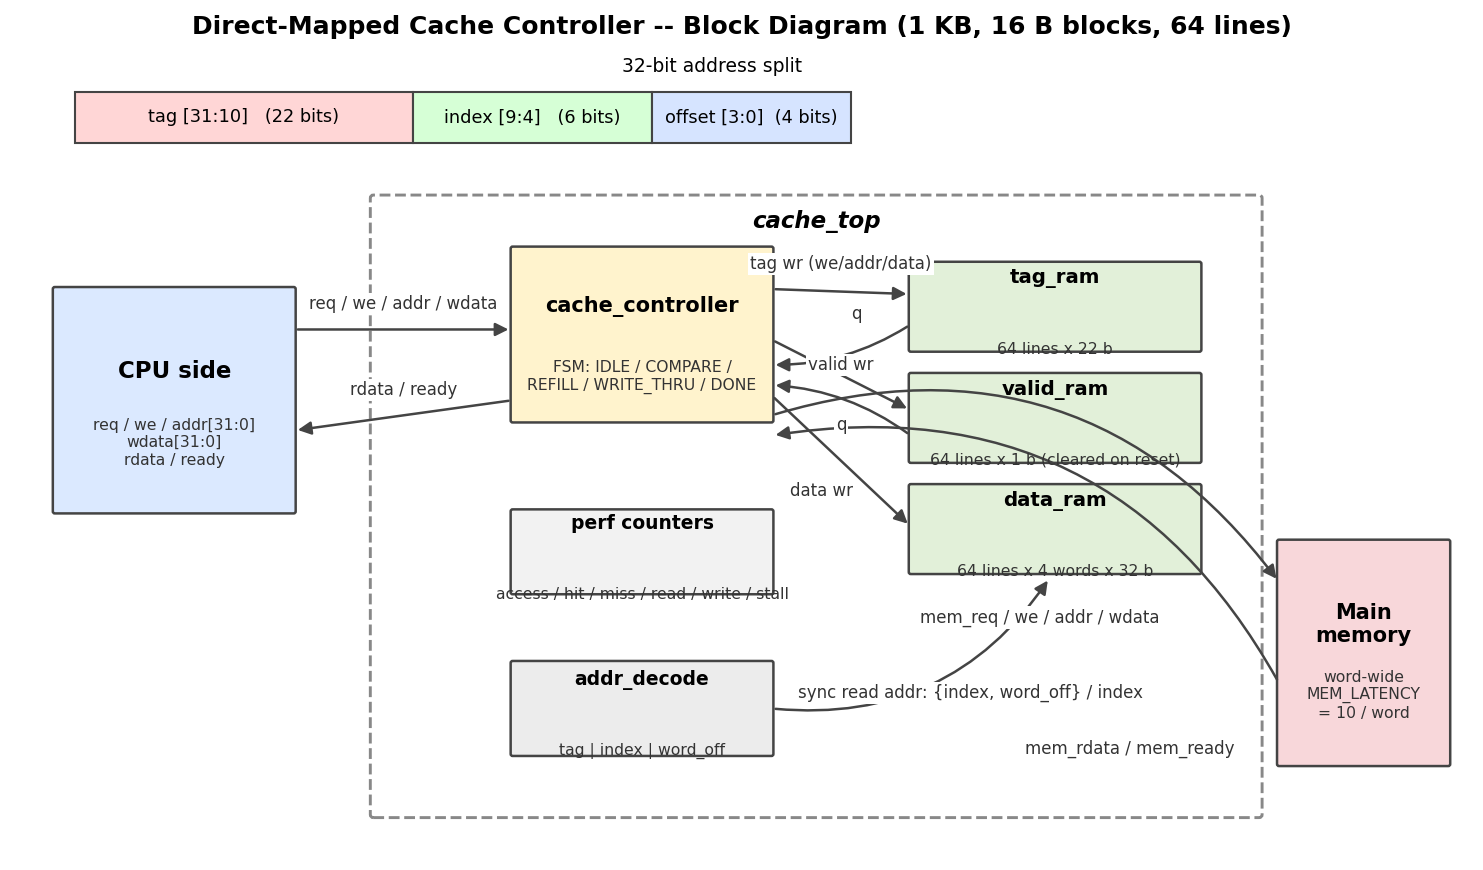
\includegraphics[width=\columnwidth]{../block_diagram.png}
  \caption{Top-level block diagram of \texttt{cache\_top}.}
  \label{fig:block}
\end{figure}

\subsection{Controller FSM}
The main control flow is illustrated in Figure~\ref{fig:fsm}. The
implemented RTL also includes the REFILL\_GAP handshake state, as
described in Table~\ref{tab:fsm}.

\begin{figure}[h]
  \centering
  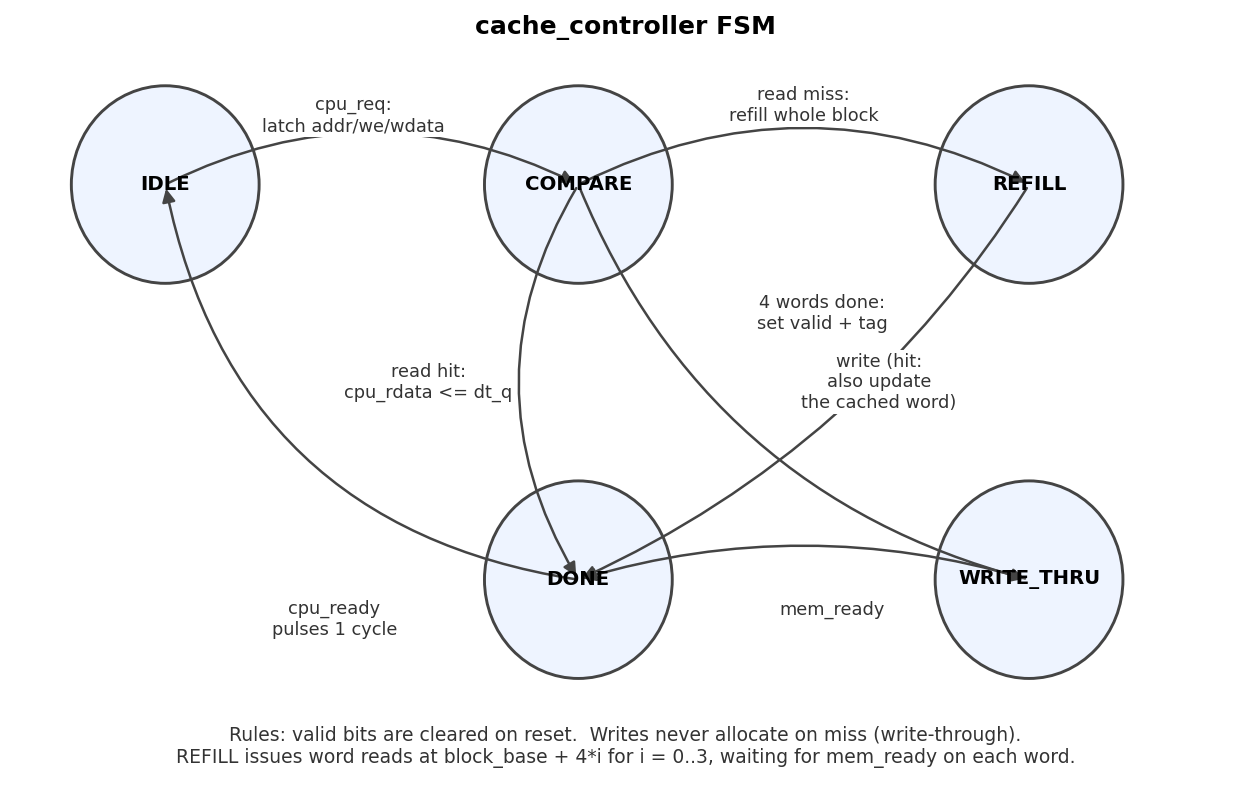
\includegraphics[width=\columnwidth]{../fsm.png}
  \caption{Cache controller FSM.}
  \label{fig:fsm}
\end{figure}

\begin{table}[h]
  \caption{FSM State Descriptions}
  \label{tab:fsm}
  \centering
  \begin{tabular}{p{1.5cm}p{3.0cm}p{2.5cm}}
    \toprule
    \textbf{State} & \textbf{Action} & \textbf{Next State} \\
    \midrule
    IDLE &
      Wait for \texttt{cpu\_req}; latch addr, we, wdata &
      COMPARE \\
    COMPARE &
      Compare tag and check valid; determine hit/miss &
      read hit $\to$ DONE;\newline
      read miss $\to$ REFILL;\newline
      write $\to$ WRITE\_THRU \\
    REFILL &
      Fetch words 0–3 from memory (block base + 4$i$); write into
      data RAM; set valid and tag &
      REFILL\_GAP between words; DONE after word 3 \\
    REFILL\_GAP &
      Deassert the memory request for one cycle before the next word &
      REFILL \\
    WRITE\_THRU &
      Issue memory write; wait \texttt{mem\_ready}; on hit update
      cached word &
      DONE \\
    DONE &
      Assert \texttt{cpu\_ready} for one cycle; output
      \texttt{cpu\_rdata} &
      IDLE \\
    \bottomrule
  \end{tabular}
\end{table}

\subsection{Module descriptions}

\paragraph{addr\_decode.v}
Combinational module that extracts tag, index, and word-select
from \texttt{cpu\_addr[31:0]}.

\paragraph{tag\_ram.v}
Synchronous register array, $64\times22$ bits.
Write-enable controlled by the FSM on refill or write-hit.

\paragraph{valid\_ram.v}
Synchronous register array, $64\times1$ bit.
Reset clears all valid bits; set by FSM after refill completes.

\paragraph{data\_ram.v}
Synchronous register array, $64\times128$ bits (four 32-bit
words per line).
Words are written individually during refill, or the hit word
is updated on a write-hit.

\paragraph{cache\_controller.v}
Five-state Mealy FSM implementing the control logic.
Drives \texttt{mem\_req}, \texttt{mem\_we}, \texttt{mem\_addr},
\texttt{mem\_wdata}; latches \texttt{mem\_rdata} on each
\texttt{mem\_ready}.
Increments six performance counters on the appropriate
transitions.

\paragraph{main\_memory\_model.v (testbench)}
Behavioural memory, word-addressable, 32-bit wide.
Initialised with $\texttt{mem}[i] = i \times 4 +
\texttt{32'hA5000000}$.
Asserts \texttt{mem\_ready} after \texttt{MEM\_LATENCY} clock
cycles.

\subsection{Verification strategy}
Directed tests in \texttt{tb\_cache\_basic.v} exercise:
(1)~cold miss and 4-word refill,
(2)~hit after refill (same address, then adjacent offset),
(3)~same-index conflict miss (evicts current block),
(4)~write-through (Phase~I: in progress).

The Python reference model (\texttt{scripts/cache\_model.py})
independently simulates the same address sequence and reports
hit/miss counts.
Phase~II will automate a \texttt{make crosscheck} target that
compares RTL counter outputs with the Python model on all five
trace files.

% ============================================================
\section{Results and Discussion}
\label{sec:results}

\textit{Note: Full RTL results will be populated in Phase~II once
\texttt{make regress} and \texttt{make crosscheck} pass.
The numbers below are from the Python reference model only and
serve as sanity checks.}

Table~\ref{tab:hitrates} shows the hit rates produced by
\texttt{scripts/cache\_model.py} on the five 10,000-access trace
files included in the repository.

\begin{table}[h]
  \caption{Python Reference Model Hit Rates (Phase~I)}
  \label{tab:hitrates}
  \centering
  \begin{tabular}{lrrrr}
    \toprule
    \textbf{Trace} & \textbf{Accesses} & \textbf{Hits} &
    \textbf{Misses} & \textbf{Hit Rate} \\
    \midrule
    loop       & 10,000 &  9,968 &    32 & 99.68\% \\
    matmul     & 10,000 &  8,885 & 1,115 & 88.85\% \\
    sequential & 10,000 &  7,500 & 2,500 & 75.00\% \\
    random     & 10,000 &     12 & 9,988 &  0.12\% \\
    stride     & 10,000 &      0 & 10,000 &  0.00\% \\
    \bottomrule
  \end{tabular}
\end{table}

The results match analytical expectations:
\begin{itemize}
  \item \textbf{Sequential}: four words per 16-byte block gives
    75\% hit rate ($1 - \frac{1}{4}$).
  \item \textbf{Loop} (512-byte working set $<$ 1\,KB cache):
    after a 32-line warm-up phase, every subsequent access is a
    hit, yielding $>$99\%.
  \item \textbf{Stride 64\,B}: each access falls in a new block,
    so the miss rate is 100\%.
  \item \textbf{Random} (1\,MB footprint $\gg$ 1\,KB cache):
    near-zero hit rate.
  \item \textbf{Matmul} ($16\times16$ matrices): B-matrix accesses
    have poor locality in row-major storage but A-matrix rows are
    reused, yielding a moderate 88.85\%.
\end{itemize}

AMAT estimates (using $t_{\text{hit}}=1$, $t_{\text{miss}}=41$):

\begin{table}[h]
  \caption{Estimated AMAT (Python model, Phase~I)}
  \label{tab:amat}
  \centering
  \begin{tabular}{lrr}
    \toprule
    \textbf{Trace} & \textbf{Hit Rate} & \textbf{AMAT (cycles)} \\
    \midrule
    loop       & 99.68\% & $1 + 0.0032 \times 40 = 1.13$ \\
    matmul     & 88.85\% & $1 + 0.1115 \times 40 = 5.46$ \\
    sequential & 75.00\% & $1 + 0.2500 \times 40 = 11.0$ \\
    random     &  0.12\% & $1 + 0.9988 \times 40 = 40.95$ \\
    stride     &  0.00\% & $1 + 1.0000 \times 40 = 41.0$ \\
    \bottomrule
  \end{tabular}
\end{table}

\textit{RTL waveform screenshots and crosscheck output will be
added in Phase~II.}

% ============================================================
\section{Individual Contributions}
\label{sec:contributions}

\subsection{Hardik Shreyas (lead)}
Hardik created the GitHub repository, defined the branch and
PR rules, and wrote the FSM controller
(\texttt{cache\_controller.v}) and the top-level wiring
(\texttt{cache\_top.v}).
He also authored the \texttt{Makefile} with targets
\texttt{sim}, \texttt{test\_units}, \texttt{regress},
\texttt{crosscheck}, \texttt{results}, \texttt{synth}, and
\texttt{clean}.
In Phase~II he will complete the \texttt{WRITE\_THRU} state,
add performance counters, and lead the 2-way LRU extension.

\subsection{Saman}
Saman designed and implemented the four RTL storage modules:
\texttt{addr\_decode.v}, \texttt{tag\_ram.v},
\texttt{data\_ram.v}, and \texttt{valid\_ram.v}.
Each module includes a self-checking testbench exercised by
\texttt{make test\_units}.
In Phase~II Saman will parameterise the design and optionally
add byte-enable support.

\subsection{Bhavay Goyal}
Bhavay Goyal implemented and verified the configurable behavioural
main-memory model (\texttt{main\_memory\_model.v}) and the self-checking
Phase~I read-path testbench (\texttt{tb\_cache\_basic.v}). The tests
cover a cold miss with four-word refill, repeated and same-block hits,
and same-index conflict replacement. Bounded transaction timeouts and
a global watchdog prevent broken RTL from hanging simulation. Running
\texttt{make sim} prints \texttt{ALL TESTS PASSED} only after every
required check succeeds and generates \texttt{sim/cache.vcd}.

\subsection{Priyansh}
Priyansh wrote the trace generator
(\texttt{scripts/gen\_traces.py}) producing five deterministic
10,000-access trace files, and the Python reference cache model
(\texttt{scripts/cache\_model.py}) that reports hits, misses,
and hit rate.
In Phase~II he will run all five traces on both the
direct-mapped and 2-way designs and produce comparison plots.

\subsection{Prateek Shukla}
Prateek produced the Phase~I documentation deliverables.
Specifically, he created the block diagram
(\texttt{docs/block\_diagram.png}) showing the full module
hierarchy and signal flow, and the FSM diagram
(\texttt{docs/fsm.png}) illustrating the main control-flow states and
their transitions.
He authored this IEEE report skeleton
(\texttt{docs/report/main.tex}) with all five required sections
(Abstract, Literature Review, Proposed Solution, Results and
Discussion, Individual Contributions).
He will present the final video segment covering the report,
repository structure, and Phase~II next steps.
In Phase~II (task~F-1) he will complete the full final report
including the Results and Discussion section with actual RTL
data.

% ============================================================
\section{Conclusion}
\label{sec:conclusion}

\textit{(To be completed in Phase~II once all RTL results are
available.)}

Phase~I has established the complete design specification,
RTL module hierarchy, FSM controller, directed testbench, Python
reference model, and documentation framework for the
direct-mapped cache controller.
Hit rates from the Python model match theoretical expectations
across all five trace types.
Phase~II will close the loop between RTL and reference model,
add write-path support, run synthesis, and extend the design to
a 2-way set-associative cache for performance comparison.

% ============================================================
\begin{thebibliography}{9}

\bibitem{hennessy2019}
J.~L. Hennessy and D.~A. Patterson,
\emph{Computer Architecture: A Quantitative Approach}, 6th~ed.
Morgan Kaufmann, 2019.

\bibitem{patterson2020}
D.~A. Patterson and J.~L. Hennessy,
\emph{Computer Organization and Design: RISC-V Edition}, 2nd~ed.
Morgan Kaufmann, 2020.

\bibitem{harris2022}
S.~L. Harris and D.~M. Harris,
\emph{Digital Design and Computer Architecture: RISC-V Edition}.
Morgan Kaufmann, 2022.

\bibitem{palnitkar2003}
S.~Palnitkar,
\emph{Verilog HDL: A Guide to Digital Design and Synthesis}, 2nd~ed.
Prentice Hall, 2003.

\bibitem{smith1982}
A.~J. Smith,
``Cache memories,''
\emph{ACM Computing Surveys}, vol.~14, no.~3, pp.~473--530,
Sep.~1982.

\bibitem{jouppi1990}
N.~P. Jouppi,
``Improving direct-mapped cache performance by the addition of a
small fully-associative cache and prefetch buffers,''
in \emph{Proc.\ 17th ISCA}, pp.~364--373, 1990.

\end{thebibliography}

\end{document}
